\documentclass[10pt,a4paper]{article}
\usepackage[utf8]{inputenc}
\usepackage{amsmath}
\usepackage{amsfonts}
\usepackage{amssymb}
\usepackage{fullpage}
\usepackage{verbatim}
\usepackage{graphicx}
\begin{document}

\title{Crowd density estimation from Wi-Fi positioning data in the Amsterdam Arena}
\maketitle

\begin{abstract}
\begin{comment}
We present the Amsterdam Arena project, which involves observing and managing crowd behaviour, using the Amsterdam Arena stadium as a living laboratory. The main scientific question we explore is how to detect anomalous behaviour in large crowds in real time. The main purpose is to be able to predict a possible crowd disaster and identify means to prevent it from happening. 
Human crowds are complex systems, and predicting or controlling their behaviour is challenging. Our approach involves three phases, firstly data collection from Wi-Fi and Bluetooth sensors in the stadium, secondly data analytics, and finally we aim to use simulation to make forecasts about the crowd dynamics. 
Here we present initial results on the data analytics and show how we can extract density maps from Wi-Fi positioning data. The technology we deploy is based on the Wi-Fi signals from smart phones. We use the existing network of Wi-Fi access points in the stadium, and capture probe signals from smart phones, which are processed and anonymised in alignment with privacy concerns. The positions of smart phones are reconstructed using received signal strengths and methods similar to trilateration. The data provides us with real-time information on spatial distributions of crowd density, which is an essential indicator of the criticality of crowd conditions. To visualise the spatiotemporal behaviour of crowd density in real-time we dynamically generate heat maps along a moving time interval. The heat maps are generated through the statistical modelling of the positioning data. The generation of dynamic heat maps allows us to detect and locate hot-spots of density where crowd conditions reach critical values that could possibly lead to a disaster.
\end{comment}
\end{abstract}

\section{Introduction}


***********************************From Sonja. nb: the text will be polished in the final phases, first I care only about putting all ideas on paper***************

Crowd disasters have taken many human lives. The Love Parade disaster (Duisburg, 2010), the Ellis Park Stadium disaster (Johannesburg, 2001), the PhilSports Stadium stampede (Manila, 2006) are just a few recent examples. One of the reasons that disasters happen is a "lack of overview of everybody" [cite paper on love parade EPJ DS], that is, a lack of macroscopic overview of the crowd. Critical crowd density (cite paper 8/m2, find it in e-mails)) is a contributing factor to crowd disasters; yet, it is still challenging to determine timely when it occurs, so that a disaster can be prevented before it happens, by e.g. navigating the rest of the crowd away from the congestion. 

In our work we are interested in estimating crowd density during concerts in indoor spaces. A lot of research on estimating crowd density has been done using video processing from security cameras (cite papers (1), (2), (3) from proposal?). However, this approach does not apply in our case, because 1)  it is difficult to obtain macroscopic overview ; 2) the lighting conditions during concert hours are not sufficient for video-based crowd analysis; and 3) the error of video-based density estimation increases with the increase of the actual crowd density.  

In our approach, we combat the three above mentioned issues by exploiting the ubiquity of smart phones, as in ((4) (5), (6) from proposal?). Our living laboratory is the Amsterdam Arena(citation). Or methodology consists of three steps.  First, we are using the Wi-Fi routers in the stadium to gather the strengths of the wireless antena signals from individuals smart phones.  Second, we are estimating anonymously the positions of the visitors from the signal strengths in real time. This technique has been presented in (cite Jan's slides), and is similar to trilateration, that is, the way the Global Positioning System (GPS) is implemented. However, due to signal interference and blockage in dense crowds, irregular internet packet rates and systematic errors leading to multiple local optima, the positioning itself does not suffice to estimate the crowd density. Thus, in our third step, we aggregate the results from the positioning and apply the law of the large numbers to obtain an estimation of the crowd density, also in real-time. With the first two steps, we are dealing with issues 1) and 2) mentioned above. With the third step, which is the main contribution of this paper, we are handling issue 3) -  that is, with our method the precision of estimation actually increases as the crowd density increases. 

The rest of the paper is organized as follows.....



************************************end from Sonja
\begin{comment}
\begin{itemize}

\item Background\\

Human crowds are complex systems, and predicting or controlling their behavior is challenging. Our approach involves three phases, firstly data collection from Wi-Fi and Bluetooth sensors in the stadium, secondly data analytics, and finally we aim to use simulation to make forecasts about the crowd dynamics. 

In this paper we present initial results on the data analytics and show how we can extract density maps from Wi-Fi positioning data. 

\item Aims\\

The main purpose is to be able to predict a possible crowd disaster and identify means to prevent it from happening. 

\end{itemize}
\end{comment}

\section{Positioning of visitors using Wi-Fi sensors and smart phones}


This section will be written later, maybe with input from Jan.

\begin{comment}
The technology we deploy is based on the Wi-Fi signals from smart phones. We use the existing network of Wi-Fi access points in the stadium, and capture probe signals from smart phones, which are processed and anonymised in alignment with privacy concerns. The positions of smart phones are reconstructed using received signal strengths and methods similar to trilateration. 


\begin{itemize}
\item How are the uncertainties (errors) generated and what do they mean?
\end{itemize}
\end{comment}
\section{From positioning to estimation of density}



\subsection{Issues with positioning (title to reconsider)}

Under ideal circumstances, the positioning itself would suffice to estimate the crowd density per region of interest:  every few seconds we would only need to count the number of estimates that fall in the region of interest. However, we have observed several issues, which are not related to the mathematical methodology behind the positioning step, that prevent us to apply direct counting. 
\begin{enumerate}
	\item
	{\it Bimodal distributions of coordinates estimations}. We have sampled randomly 20 MAC addresses and plotted the estimations of their coordinates through time, where we have plotted only the estimations with a relatively small uncertainty. We observed persistent bimodal distribution of the estimations, an example of which can be seen in Fig. \ref{fig:bimodal}. 
		\begin{figure}[h!]
			\centering
			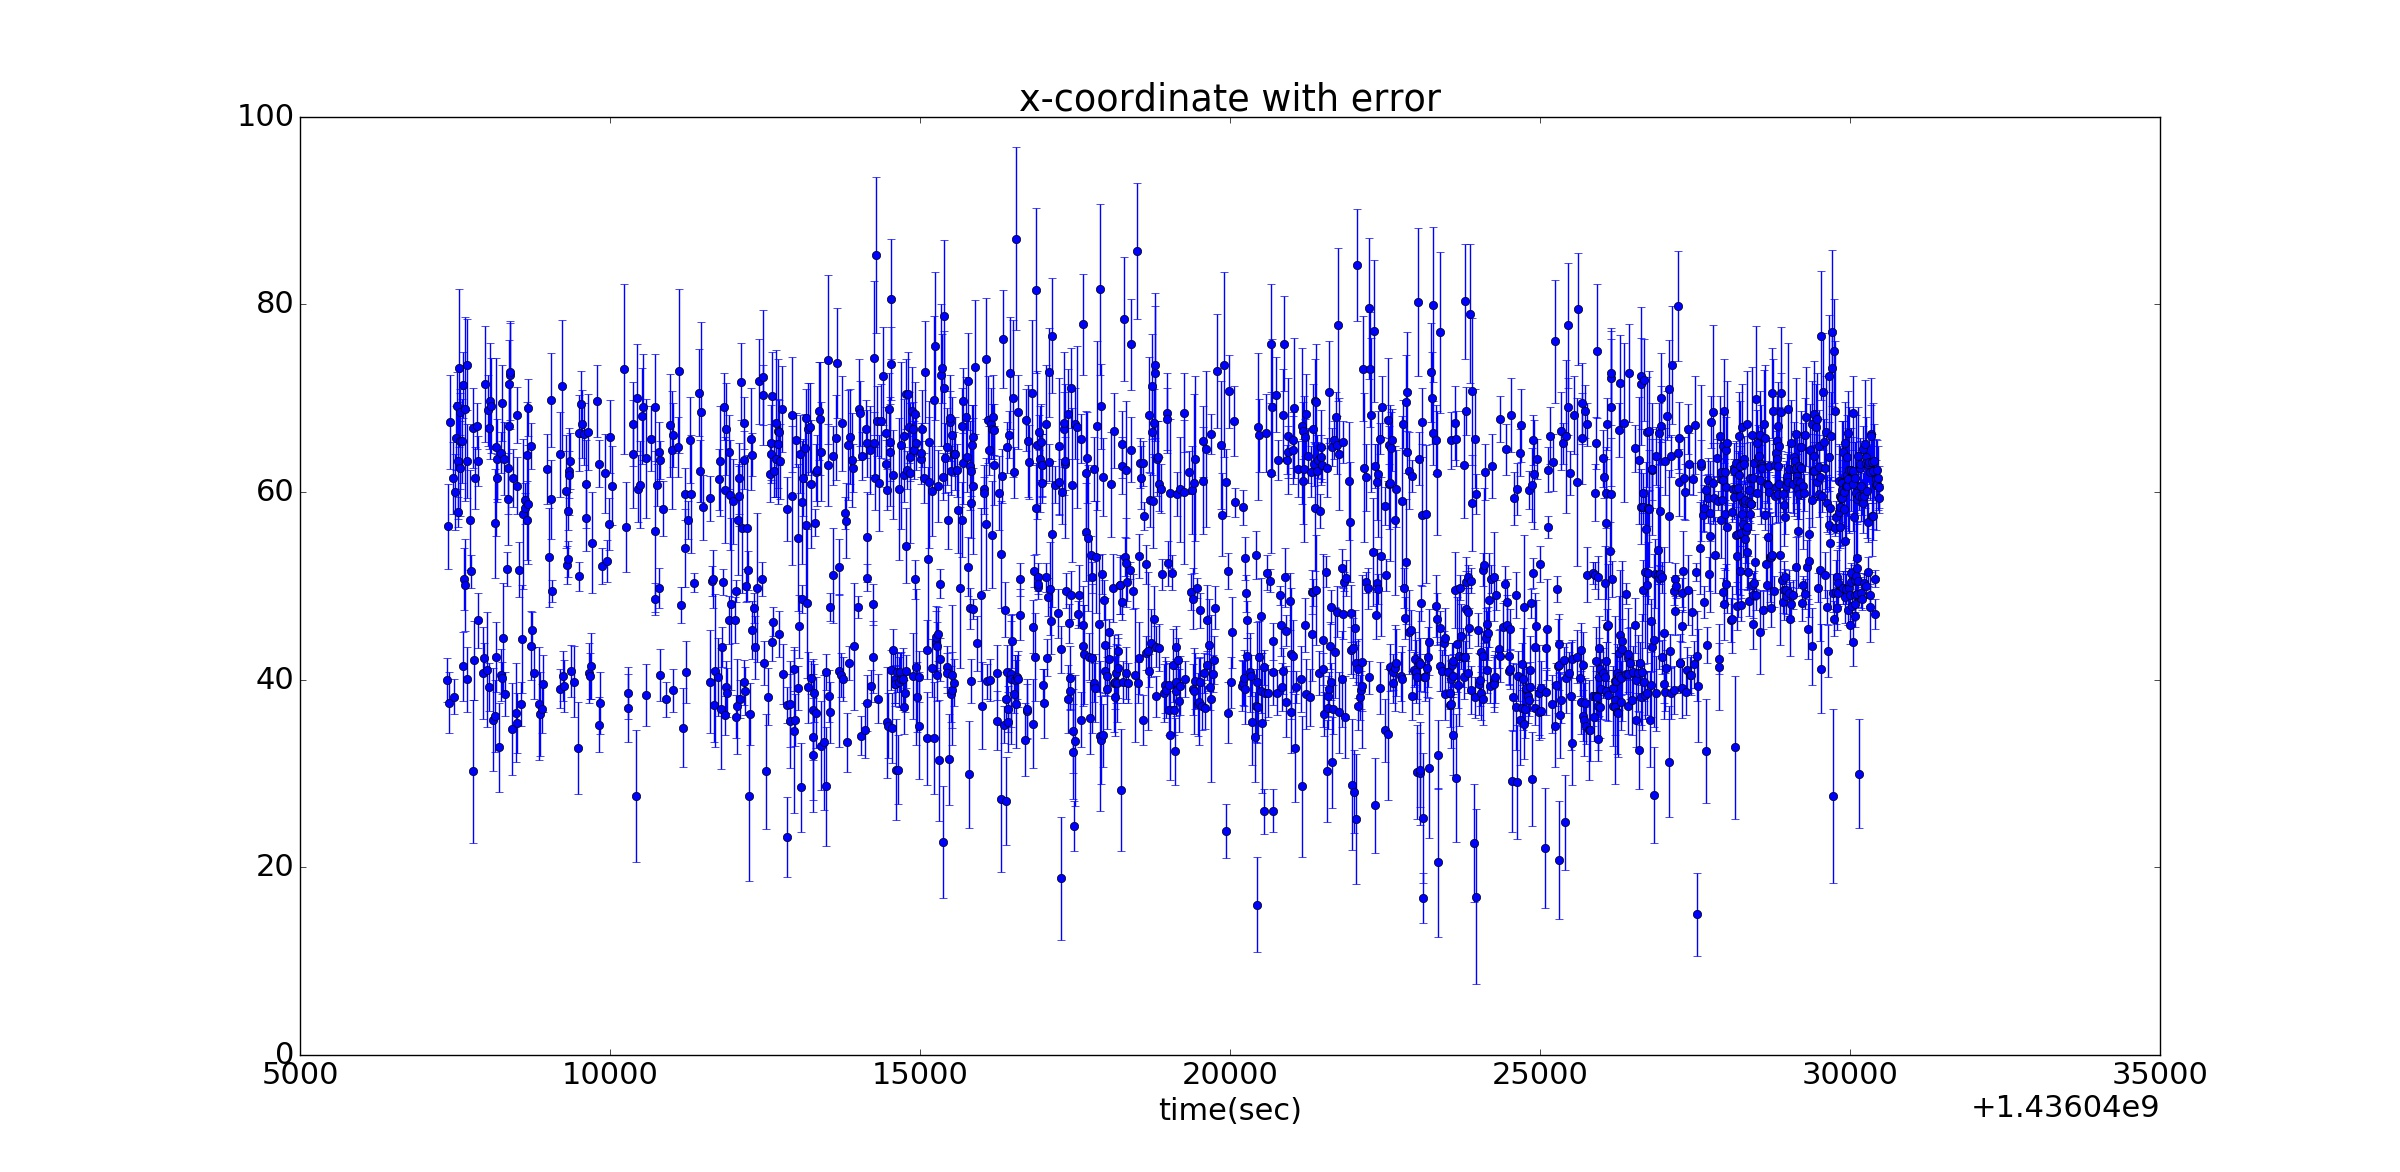
\includegraphics[width=120mm]{bimodal.jpg}
			\caption{Estimation of x-coordinate of a static MAC device through time with error}
			\label{fig:bimodal}
		\end{figure} 
	This figure shows the estimated x-coordinates through time of a static, 24 hours persistent MAC address. Because we did not observe  bi-modal distributions in the signal strengths, the bi-modal distribution of the positions estimates can be explained by the multiple local optima situation. Namely, due to signal interference, when the optimization of the estimation of location of a certain MAC address is performed, there can be multiple local optima that are equally good candidates. For example, consider Fig. \ref{fig:trilateration_problem} \footnote{Picture courtesy of http://math.stackexchange.com/questions/42537/trilateration-with-bounds}. In the center of every ring there is a Wi-Fi router, that has estimated signal strength to a certain MAC device with a certain error range. The error range is represented by the thickness of the ring. Then, there are two possible regions which are equally good candidates for the positioning of the MAC device, and those regions are the two darkest regions where all three rings overlap. Note that the problem can arise regardless of the thickness of the rings or the number of Wi-Fi routers. 	
	\begin{figure}[h!]
		\centering
		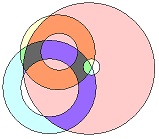
\includegraphics[width=40mm]{trilateration_problem.jpg}
		\caption{Trilateration can lead to multiple local optima}
		\label{fig:trilateration_problem}
	\end{figure}
	
	
\item {\it Volatility of packet rates}. When a MAC device is connected to the WI-Fi internet, it sends packets with a relatively stable rate. However, during concert hours, very few devices are actually connected to the internet, and most of our estimations of positions come from signals that the device sends in a "probing" mode. In this case the packet rate is quite volatile, ranging from a few seconds to a few minutes (some citation?). This means that when we make a snapshot of the MAC addresses visible in a certain moment, we are only detecting a small fraction of the MAC devices.   

\item {\it MAC randomization}. Due to ever increasing privacy concerns and possibly other business reasons, starting from 2014, the Apple I-phones have introduced randomization of the MAC address when the device is in a probing mode (not connected to internet) (citation?). This means that when the device switches from a probing to an online mode or vice versa, the MAC address suddenly changes and thus the device cannot be followed anymore. It is worth noting, however, that the MAC address comes with a tag that reveals whether the address belongs to a certain domain (is non-randomized) or is randomized.    
\end{enumerate}


\subsection{Addressing the issues: real-time crowd density estimation}

\subsubsection{Issue 1: creating a statistical ensemble}
*************from Sonja

In order to deal with issue 1 from above, let us start with the following observation: we are not interested in the individual locations of the MAC devices, but rather in the density of the crowd; we would like especially to have more precise estimation when the density reaches a certain threshold, so that the crowd that is not in the dense region can be alarmed promptly to move away from the dense region.
This situation, dense crowd, means that there is more blockage of signals from bodies, less precise estimation of distance from Wi-Fi based on signal strength, which means that the rings in Fig.\ref{fig:trilateration_problem} would be even thicker. This exaggerates the effect of "bimodal" or even multi-modal distribution of position estimates. Thus, in a dense crowd, all we can derive from the positioning method for a MAC device is a probability distribution of its possible locations. For example, in the scenario in Fig. \ref{fig:trilateration_problem}, we can say that the MAC device is with a probability of 0.5 in the left grey region (region where all three rings overlap) and with a probability of 0.5 in the right grey region. While this does not provide us with useful information for the location of the MAC device, if we apply the same reasoning for all MAC devices, and, for a region R we add together the probabilities for all MAC devices that they are in that region, we end up with an estimation of the number of MAC devices in that region. If we assume that the locations of the MAC devices are mutually independent, we can  apply directly the law of the large numbers and conclude that for a dense crowd the error of the estimation of the density per region will vanish. However, we cannot assume the mentioned independence, because people tend to go in groups to concerts. In this case, the variance of the estimation is equal to the average correlation between the locations in the limiting case. Nevertheless, we can safely assume that for a regular crowd at a concert the average correlation tends to zero as the number of people increases; thus, the error of the estimation of the crowd density will in anyway diminish as the number of people tends to infinity. 

Formally, 
let $\{mac_1, mac_2,...mac_n\}$ be all MAC devices detected at time $t$. Let $R$ be an arbitrary region from the stadium.  Let $X_i$ be a random variable defined by

$$X_i = 
\left\{
\begin{array}{ll}
1  & \mbox{if } mac_i \in R \\
0 & \mbox{if } mac_i \notin R
\end{array}
\right.  $$

 Denote by $X$ the total number of devices in $R$ detected at time $t$. Clearly, $X=\sum_{i=1}^{n} X_i$.
Then $E(X)$, the expected value of $X$ is $$ E(X) = E(\sum_{i=1}^{n} X_i) = \sum_{i=1}^{n}E( X_i) = 
\sum_{i=1}^{n}(1\cdot Prob(mac_i \in R) + 0 \cdot Prob(mac_i \notin R)) = \sum_{i=1}^{n} Prob(mac_i \in R) ,$$
where by $Prob(mac_i \in R)$ we denote the probability that $mac_i$ is in the region R at time $t$.
We postpone the derivation of $Prob(mac_i \in R)$ a bit. 

Next, we show that the variance of $X/n$, that is, the number of devices in $R$ normalized w.r.t the total number of detected devices, diminishes when $n$ becomes large (the variance of $X$ in the limiting case is out of our interest because then $E(X)$ is potentially infinite). This suffices to show that our method of estimation of crowd density is theoretically sound, given the probabilities $Prob(mac_i \in R)$. We have

\begin{equation}\label{eq_Var}
Var(\frac{X}{n} ) =  Var(\frac{1}{n} \cdot \sum_{i=1}^{n} X_i) = \frac{1}{n^2} \cdot Var(\sum_{i=1}^{n} X_i) = \frac{1}{n^2} \cdot (\sum_{i=1}^{n} Var(X_i) + \sum_{i \not =  j}Cov(X_i,X_j))
\end{equation}


We can assume that there is an upper limit $\lambda$ of a number of people that go to a concert together (a group), that is, whose locations are correlated\footnote{Actually, when the crowd is so dense that people can not move freely anymore, the whole crowd becomes a "group" (cite LP disaster) and all locations are correlated. But we aim to detect a high density with our method {\it before} this happens, to react preventively; otherwise, it is too late.}. Denote by $\kappa$ the maximal covariance between any $X_i$ and $X_j$ and let us write $i \sim j$ if and only if $i$ and $j$ are in the same group. 
Then, 
\begin{equation}\label{eq_covar}
\sum_{i \not =  j}Cov(X_i,X_j) = 2 \sum_{1\leq i <  j \leq n }Cov(X_i,X_j) =  2 \sum_{i,j: i \sim j }Cov(X_i,X_j)  \leq 2 n \cdot \frac{\lambda(\lambda - 1)}{2} \cdot\kappa = n  k \lambda(\lambda - 1)
\end{equation} 
where the inequality holds because the maximal number of groups is $n$ and the maximal number of pairs $(i,j)$ in a group is $\lambda(\lambda-1)/2$.
Let $\mu = \frac{1}{n}\sum_{i=1}^{n} Var(X_i)$, that is, 
denote by $\mu$ the average variance of $X_i$.  From \eqref{eq_Var} and \eqref{eq_covar} we have  

\begin{equation}
Var(\frac{X}{n} ) \leq \frac{1}{n^2}(n \mu + n  k \lambda(\lambda - 1)) = \frac{1}{n}(\mu +  k \lambda(\lambda - 1)), 
\end{equation}
which tends to $0$ when $n \rightarrow \infty$. Note that we have greatly overestimated the variance with the inequation in \eqref{eq_covar}. 

Next, we can proceed with derivation of $Prob(mac_i) \in R$ for arbitrary $i$ in order to evaluate $E(X)$. 
   
**** below: in the kernel function there is a typo:  the negative sign in front of $u^2$ is forgotten
***************end from Sonja

***start from Philip

\begin{comment}
To visualise the spatiotemporal behaviour of crowd density in real-time we dynamically generate heat maps along a moving time interval. The heat maps are generated through the statistical modeling of the positioning data. The generation of dynamic heat maps allows us to detect and locate hot-spots of density where crowd conditions reach critical values that could possibly lead to a disaster.
\end{comment}

The data provides us with a series of estimated positions of mobile devices, together with their corresponding values of measurement uncertainty (see Section on Positioning).
\begin{comment}
The uncertainty values are determined by the co-variance matrix resulting from the chi-square fitting method.
\end{comment}
From this data we wish to estimate crowd density distributions, along a moving time window.
So, our first step is to select from the data estimated positions whose time stamps fall within a specified time interval $[t-\Delta t,t]$.
From the selected estimated positions we then construct density estimates for the individual mobile devices, and add them up to construct the crowd density distribution.

A natural way to construct density estimates for the individual devices would be to construct density histograms, by binning the estimated positions.
However, in constructing the density estimates we wish to preserve and visualize the uncertainty that corresponds to each estimated position.
Therefore, we smooth each position into a bivariate Gaussian `bump', using the uncertainty values ($\sigma_{x}$ and $\sigma_{y}$) provided by the data.
For each detected MAC address we construct a two-dimensional density estimate by adding up these smoothed positions, which we normalize by the number of measurements $N$ we have for that MAC address in the selected time window.
Thus, the density estimate for a mobile device is the sum of a series of Gaussian `bumps' with variable width, centered at the estimated positions.

Finally, to construct our crowd density estimation we sum the individual density estimates of all the devices.
This estimated crowd density distribution integrates to the number of MAC addresses detected in the time window.

The implementation of our method is similar to that of kernel density estimation \cite{scott}\cite{silverman}.
In our case the amount of smoothing is variable and determined by the measurement uncertainty values $\sigma_{x}$ and $\sigma_{y}$.
The density estimate for a mobile device $m$ at a location $(x,y)$ is defined by

\begin{equation}
\hat{f}_{m}(x,y)=\frac{1}{N}\sum_{i=1}^{N}K((x-x_{i}),\sigma_{x}) K((y-y_{i}),\sigma_{y})
\label{kde}
\end{equation}
where $N$ is the number of measurements (positions) for MAC address $m$, and the kernel function $K$ is given by
\begin{equation}
K(u,\sigma)=\frac{1}{\sigma\sqrt{2\pi}}\exp(\frac{u^2}{2\sigma^2})
\end{equation}
The final crowd density estimation is given by
\begin{equation}
\hat{f}_{T}(x,y)=\sum_{m}\hat{f}_{m}(x,y)
\label{total}
\end{equation}

\begin{comment}
\subsection{Real-time data analysis}

To process positioning data in real-time during events, we consider data within a specific moving time window.
To take in account that visitors are moving, we subdivide the time window in multiple sub-windows and attach more weight to measurements in later sub-windows. The weighting scheme is given by

\begin{equation}
\hat{d}(X,t)=\frac{w_{1}\hat{f}(X,t_{1})+w_{2}\hat{f}(X,t_{2})+...+w_{m}\hat{f}(X,t_{m})}{w_{1}N_{1}+w_{2}N_{2}+...+w_{m}N_{m}}
\end{equation}

\noindent where $\hat{f}(X,t)$ is the non-normalized sum of smoothed counts ($N\times\hat{d}(X,t)$) in Equation \ref{kde}, $w_{k}$ is the weight value given to sub-window $k$, and $m$ is the number of sub-windows.
\end{comment}

\subsubsection{Issue 2: Conservation of mass }
****************begin from Sonja

To address the second issue {\it Volatility of packet rates}, we ensure that we do not forget about the MAC devices that were not observed in the last time window. In fact, for every MAC device that was ever observed, until it has been observed again we maintain the old probability distribution, too. Over time this probability distribution turns gradually into a uniform by smoothing it every epoch with a Gaussian kernel. The size of the kernel changes over time and is related to the maximal speed that the MAC device can have under the current density distribution of the crowd. In other words, we assume a Brownian motion of the MAC device, where the speed is limited by the maximal speed of a pedestrian under the current crowd conditions (cite paper Johansson et al). When the MAC device is observed again, its old probability distribution is simply overwritten by the probability distribution that is computed as above. 

Formally,  (now write formulas) 

****************end from Sonja\\

\begin{comment}
below is a first sketch, nothing definite yet
\end{comment}

For the epochs during which a mobile device is not detected we assume Brownian motion (without drift), which is defined by

\begin{equation}
\text{d}X(t)=\sqrt{2D}\text{d}W(t)
\end{equation}
where $W(t)$ is a Wiener process. The density function $f(t,x)$ of the displacement of $X$ in the time interval $[0,t]$ is known, and is a normal distribution with mean $X(0)$ and variance
\begin{equation}
\sigma^2=2Dt
\end{equation}
Thus, in case have no new observations, we can further smooth the density estimate from the previous epoch by convolution with a normal distribution. 
The variance is determined by the length $t$ of the time interval, and the (average) walking speed of pedestrians. The walking speed in turn can be related to the local crowd density via the so-called fundamental diagram.\\

\subsubsection{Issue 3: using Big data again}

***************begin from Sonja

To address the last issue, {\it MAC address randomization}, we rely once again on the fact that we have a lot of data. Namely, we know from the structure of the MAC address whether it is randomized or not. Figure \ref{fig:randomized} shows the ratio between randomized and non-randomized addresses observed per minute from midnight until 6:00 am. We can see that it is quite stable through time; in fact, the Pearson correlation coefficient between the time series of randomized and non-randomized addresses is 0.88. 

\begin{figure}[h!]
	\centering
	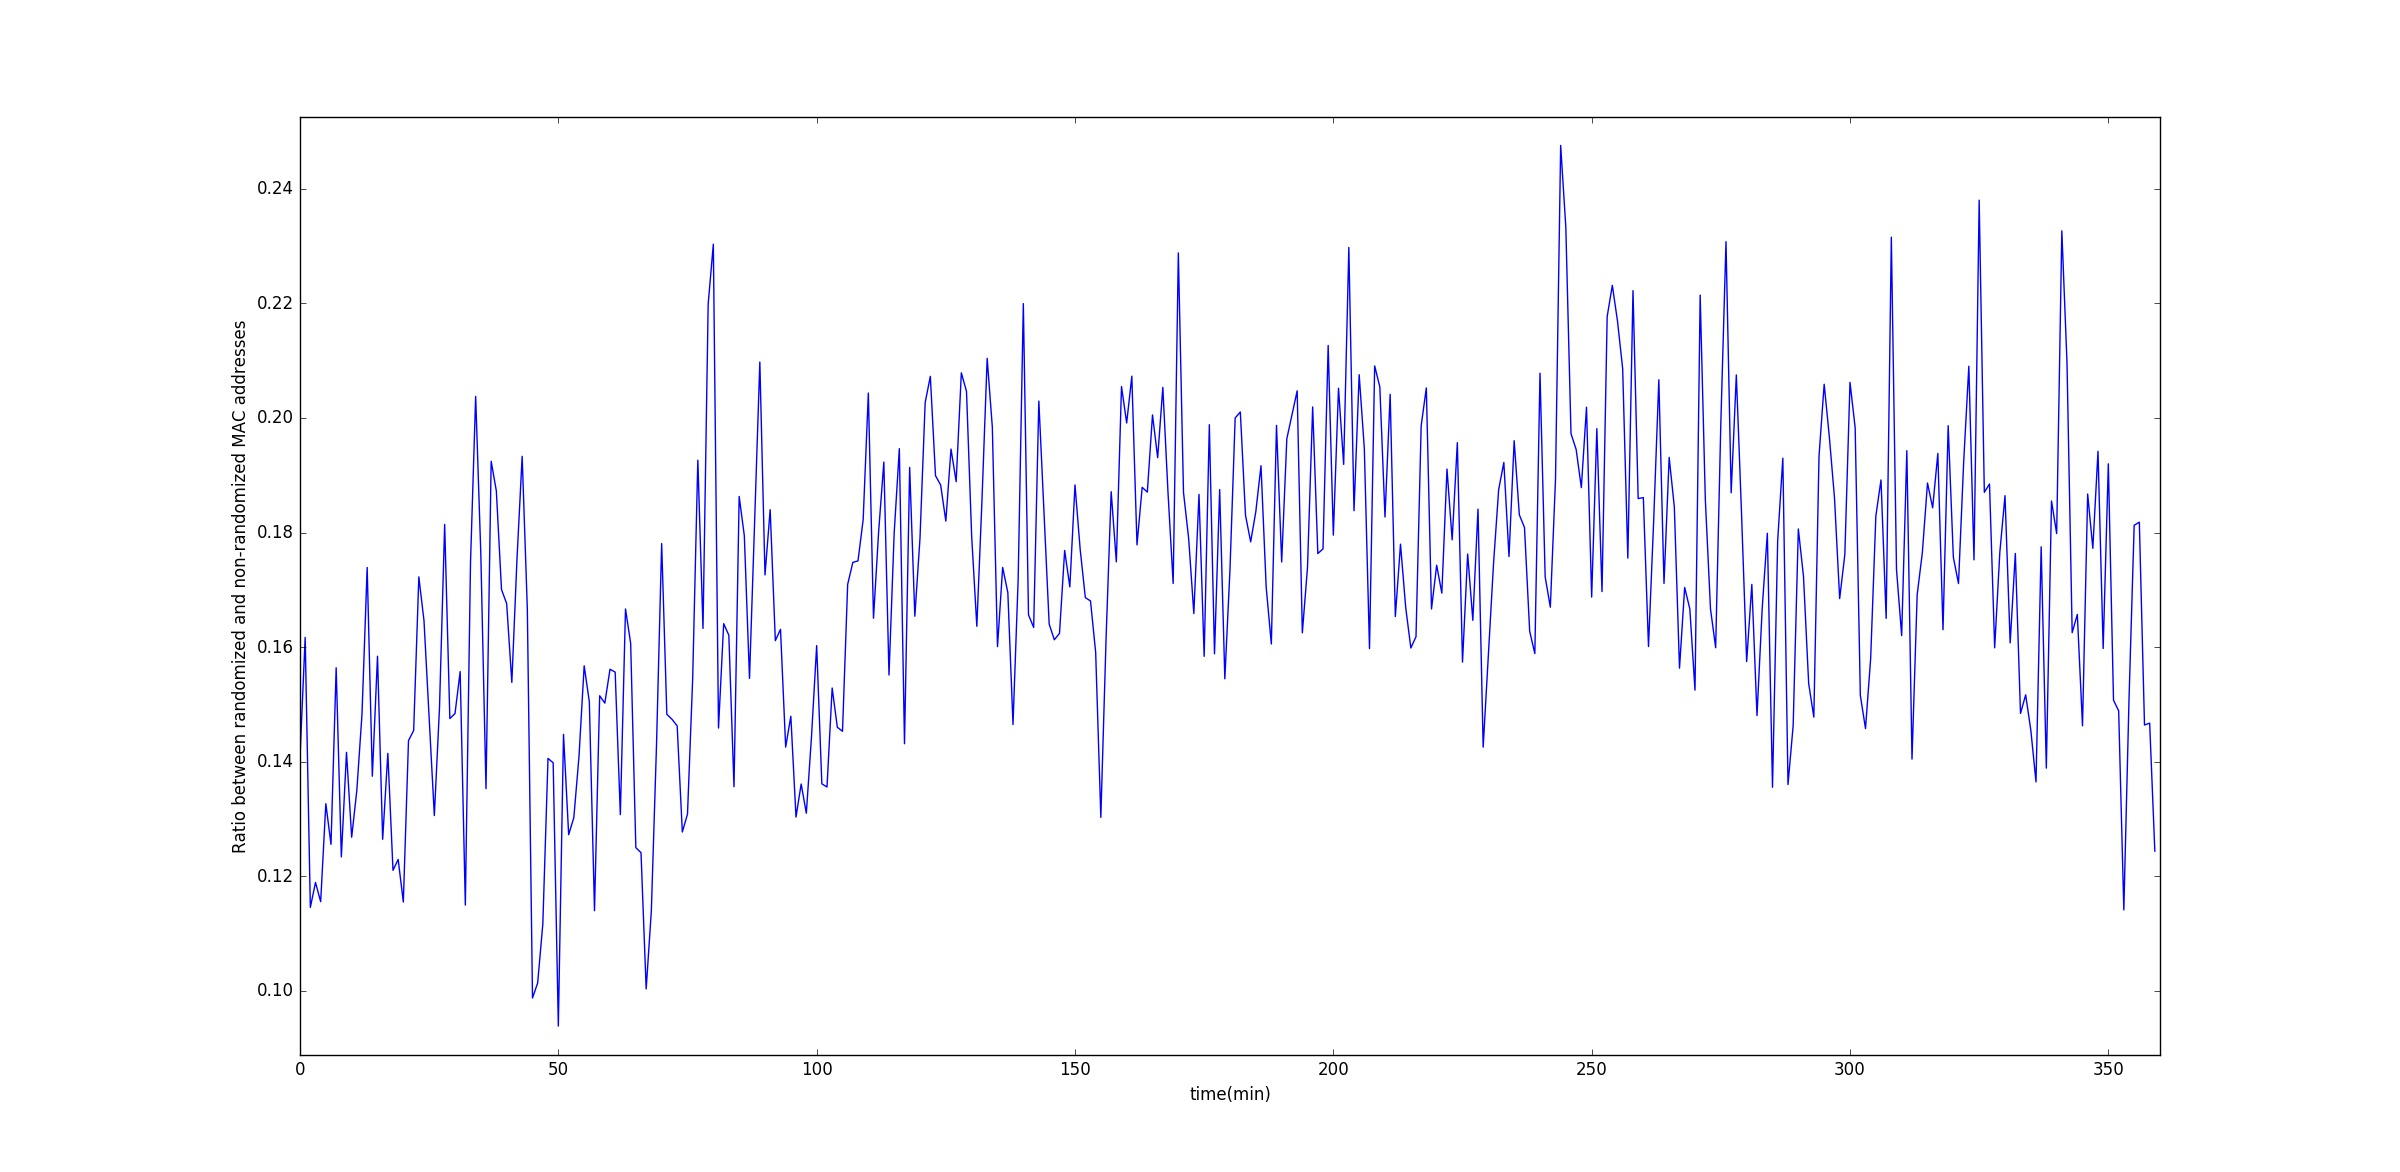
\includegraphics[width=130mm]{RatioRandNonrand.jpeg}
	\caption{Ratio between randomized and non-randomized addresses observed per minute}
	\label{fig:randomized}
\end{figure} 

Thus, when estimating crowd density, we ignore the MAC devices that have a randomized address and at the end we multiply the crowd density by 1.225, to account for the ignored MAC devices. We choose factor 1.225 to allow for a safety margin: in the peaks of the graph in Fig. \ref{fig:randomized} the values are 0.225, and we would rather overestimate than underestimate the crowd density. 
Note that this ratio should be re-computed periodically, to account for the changing conditions at the smart phones market. 
********mention the absolute numbers, or give graphs)
*******end from Sonja


\subsection{Validation}
Maybe with crowd sourcing images and videos from Sensation 2015 Amsterdam White


\section{Related work}

Wirz \textit{et al.} (2012) \cite{wirz:1} infer crowd density from GPS location traces of people who use an App during the 2011 Lord Mayor Show in London. They visualize the data in real-time, and generate heat maps (dynamically) using the kernel density estimation (KDE) method. In (Wirz \textit{et al.} 2013) \cite{wirz:2} the methodology is presented more elaborately, using a real-world data set collected during the same festival. The relation between the number of App users and the crowd density is calibrated (using linear regression), which forms the basis of their participatory sensing method. **********from Sonja: but the main idea/proposition in this paper is that they are reverting the formula for speed as a function of density of Johansson, to infer the density when they know the speed (??)******end from sonja*****
The accuracy of the smoothing method is assessed using ground truth crowd density information obtained from video footage recorded by CCTV cameras. 
The influence of the kernel radius on the correlation between the actual density and the density of App is analysed.

The Gaussian weight function used in (Wirz \textit{et al.} 2012; 2013) \cite{wirz:1}\cite{wirz:2} is introduced in Helbing \textit{et al.} (2007) \cite{helbing:1} to estimate local densities in an area captured by video cameras during the Hajj in Mina/Makkah in 1426H on January 12, 2006.\\

A number of studies use Bluetooth to estimate crowd densities at a wide range of places and events.
In these studies the position of a mobile phone is approximated to the location of the sensor by which it is detected.

Schauer \textit{et al.} (2014) \cite{schauer:1} count unique MAC devices detected by two sensors (nodes) at both sides (public and security) of a security check inside a major German airport, to estimate pedestrian densities and pedestrian flow. They consider time information, to determine the direction of a person's movement, and at least one RSSI value, to reduce the number of false positives in case devices are captured by both sensors. They compare Bluetooth and Wi-Fi based methods, and compare their methods to a known ground truth provided by the number of security checks.

Versichele \textit{et al.} (2012) \cite{versichele:1} use Bluetooth scanners at strategic locations during the 10-day Ghent Festivities, to analyze spatio-temporal dynamics of pedestrians. 

Yoshimura \textit{et al.} (2016) \cite{yoshimura:1} use Bluetooth detection to analyze visitors' behavior at the Louvre museum in Paris.

Delafontaine \textit{et al.} (2012) \cite{delafontaine:1} use a similar approach (of Bluetooth tracking) and apply (genetic) sequence alignment methods to analyze the resulting data which consists of different sequences of sensors (nodes) for detected mobile devices.

Weppner and Lukowicz (2013) \cite{weppner:1} estimate crowd densities during a soccer European championship public viewing event and during the Oktoberfest, by distributing volunteers in the crowd, who are carrying smart phones scanning for Bluetooth devices. They then use statistics to combine the different measurements in space and time.

In Weppner \textit{et al.} (2014) \cite{weppner:2} similar methods are applied to a city-wide festival in Zurich 2013, now supported by GPS data.



\section{Conclusion}

Sonja:Mention somewhere that in the documentary of the LP disaster people were raising their phones up to look for a way out. (which is good , less blockage of signals)


*************n.b. in related work section put all that use wi-fi tracking, for those that use GPS tracking only mention that this does not work in indoor spaces and that it requires participation. Not necessary to put work on video tracking in related work - it is already mentioned in intro. Mention also bluetooth tracking, but bluetooth is not so ubiquitous and our principles apply also if bluetooth was used (right?) 
Finally, none of the mentioned work uses our approach of modeling the position of an individual as a probability distribution; our method is designed to attack the problem of having a dense crowd; we are not interested in precise estimations for freely moving crowds; rather, we are interested in obtaining precise estimation when the  concert crowds is dense and static due to this. blah blah (sonja: explain better)********

Future work: indclude map of the venue in the calculations, perhaps not both dark  regions in \ref{fig:trilateration_problem} are accessible by people!

\bibliography{references}
\bibliographystyle{plain}

\end{document}